\documentclass[11pt]{article}

\usepackage[utf8]{inputenc} % Required for inputting international characters
\usepackage[T1]{fontenc} % Output font encoding for international characters
\usepackage{graphicx}
\usepackage{float}
\usepackage{hyperref}
\usepackage{amsmath}
\usepackage{cite}
\usepackage{pdfpages}
\usepackage{caption} 
\captionsetup[table]{position=above,skip=0.7cm} 
\usepackage{adjustbox}
\usepackage[german]{varioref}
\usepackage{mathpazo} % Palatino font
\usepackage[german]{babel}
\parindent0pt
\pdfinclusioncopyfonts=1

\begin{document}

\begin{titlepage} % Suppresses displaying the page number on the title page and the subsequent page counts as page 1
	\newcommand{\HRule}{\rule{\linewidth}{0.5mm}} % Defines a new command for horizontal lines, change thickness here
	
	\center % Centre everything on the page
	\vspace*{0.75cm}
%
\includegraphics[width=0.8\textwidth]{../tex/fu_logo}\\[1cm] 

%\textsc{\LARGE  Freie Universität Berlin}\\[1.5cm] % Main heading such as the name of your university/college
	
	\textsc{\Large Neurobiologie für BioinformatikerInnen: Praktikum B}\\[0.65cm] % Major heading such as course name
	
	\textsc{\large Protokoll zum 3. Praktikumstag am 21.01.2019}\\[0.65cm] % Minor heading such as course title

	\HRule\\[0.5cm]
	
	{\huge\bfseries Neurosim} \\[0.2cm]{\Large Computersimulation von Nervensignalen}\\[0.3cm] % Title of your document
	
	\HRule\\[0.75cm]
	\textsc{\Large\bfseries Gruppe V}
	\\[0.8cm]
	
\vfill

	\begin{minipage}{0.45\textwidth}
		\begin{flushleft}
			\large
			\textit{Gruppenmitglieder}\\
			\textsc{Alia Rothkegel}\\
			\textsc{Mara Steiger}
			 % Your name
		\end{flushleft}
	\end{minipage}
	~
	\begin{minipage}{0.45\textwidth}
		\begin{flushright}
			\large \vspace{16pt}
			alia.rothkegel@fu-berlin.de\\
			mara.steiger@fu-berlin.de 
		\end{flushright}
	\end{minipage}
	
\vfill

	\begin{minipage}{0.45\textwidth}
		\begin{flushleft}
			\large
			\textit{Lehrveranstalter}\\
			Prof. Dr. P.R. \textsc{Hiesinger}\\ 
			Dr. D. \textsc{Malun}\\ 
			Prof. Dr. M. \textsc{Wernet}
		\end{flushleft}
	\end{minipage}
	~
		\begin{minipage}{0.45\textwidth}
		\begin{flushright}
			
		\end{flushright}
	\end{minipage}
\vfill
	\begin{minipage}{0.7\textwidth}
		\begin{flushleft}
			\large
			\textit{TutorInnen}\\
			\textsc{Lisa Peters}\\
			\textsc{Johannes Brüner Hammacher}\\
			\textsc{Claudia Haushalter}
		\end{flushleft}
	\end{minipage}
	~
		\begin{minipage}{0.2\textwidth}
		\begin{flushright}
			
		\end{flushright}
	\end{minipage}

	% If you don't want a supervisor, uncomment the two lines below and comment the code above
	%{\large\textit{Author}}\\
	%John \textsc{Smith} % Your name
	\vfill\vfill\vfill % Position the date 3/4 down the remaining page

	
	\vfill % Push the date up 1/4 of the remaining page
	
\end{titlepage}

%----------------------------------------------------------------------------------------
\section{Einleitung}

\subsection{Membranpotential von Neuronen}
Die Fortleitung von Informationen wird von Zellen des Nervensystem übernommen und basiert auf Spannungsunterschieden zwischen dessen Zellinnerem und dem extrazellulären Raum. \\
Aufgrund der Semipermeabilität der Membran von Neuronen liegt ein sogenanntes Ruhepotential von ca. -70mV vor. Die Membran ist für größere Ionen wie Natrium ($Na^{+}$) nicht permeabel, aber Kalium ($K^{+}$) kann frei diffundieren. Daher entspricht das Ruhemembranpotential in etwa dem Gleichgewichtspotential von Kalium. Durch die geringere Konzentration von Kalium-Ionen außen ergibt sich ein negatives Membranpotential, d.h. die Nervenzelle ist gegenüber der Außenseite negativ geladen. Außerdem trägt eine Natrium-Kalium-Pumpe ($Na^{+}$-$K^+$-ATPase) zum Erhalt des Membranpotentials bei.  


\subsection{Nernst-Gleichung}
Mit Hilfe diese Gleichung lässt sich das Gleichgewichtspotential $E_{ion}$ für Ionen berechnen, d.h. das Membranpotential bei dem sich die Ionenbewegungen im Gleichgewicht befinden. Dieses Potential ist abhängig von der Ionenkonzentration außen $c_a$ und innen $c_i$. Außerdem wird vereinfachend eine Temperatur von 20 Grad angenommen. 
\begin{equation}
\label{nernst}
E_{ion} = 58mV \cdot \log(\dfrac{c_a}{c_i})
\end{equation}

Um mehrere Ionen für das Membranpotential von Neuronen zu berücksichtigen, benötigt man die komplexere Goldmann-Gleichung. Sie bezieht zusätzlich für jedes Ion die entsprechende Permeabilität der Membran mit ein. 

\subsection{Voltage-Clamp-Methode}
Um Strom durch Ionenkanäle der Nervenzellmembran zu messen verwendet man die Voltage-Clamp-Technik. Dabei wird eine Elektrode verwendet, die die Spannung an der Membran misst und mit einer Sollspannung vergleicht. Dazu wird noch eine zweite Elektrode benötigt, die entsprechende Abweichungen von der Sollspannung ausgleichen soll. Dieser benötigte Stromfluss entspricht dem Ionenstrom durch die Membran. 

\subsection{Aktionspotentiale}
Eine Nervenzelle wird durch die Bindung eines Neurotransmitters an einen ligandengesteuerten Ionenkanal in der Plasmamembran aktiviert. Dieser Kanal öffnet sich durch die Bindung, woraufhin $Na^{+}$ entlang des Konzentrationsgradienten in die Zelle einströmt und eine Depolarisation bewirkt. Spannungsabhängige $Na^{+}$-Kanäle entlang des Axons einer Nervenzelle, die durch die Depolarisation in benachbarten Regionen der Zelle kurz geöffnet werden, sorgen für die Ausbreitung des Aktionspotentials in Form einer Depolarisationswelle durch das Neuron. Kurz nach der Depolarisation durch den Natrium-Einstrom öffnen sich auch spannungsgesteuerte $K^+$-Kanäle entlang des Axons, die wiederum eine Repolarisation durch den Ausstrom von Kalium bewirken. Da diese Kalium-Kanäle etwas langsamer schließen, kommt es zu einer Hyperpolarisation der Zelle. Anschließend wird das Ruhepotential durch Leckströme von Ionen und die Aktivität der Natrium-Kalium-Pumpe wiederhergestellt.  
%\begin{figure}[H]
%\makebox[\textwidth][c]{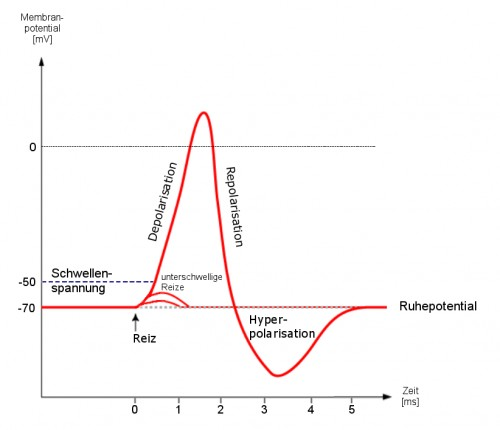
\includegraphics[width=0.85\textwidth]{aktionspotential}}
%\caption{Die Abbildung zeigt den zeitlichen Verlauf eines Aktionspotentials einer Nervenzelle. Zu sehen ist die Depolarisation von -70mV auf ca. +20mV, danach die Repolarisation übergehend zur Hyperpolarisation zu ca. 100mV und die Wiederherstellung des Ruhepotentials.  }
%\label{ap}
%\end{figure}

\subsection{Refraktärphase}\label{refraktär}
Nachdem die Natrium-Kanäle während der Depolarisation kurz geöffnet waren, sind sie für eine bestimmte Zeit inaktiviert. Diese Phase nennt man Refraktärphase. Währenddessen können diese Natrium-Kanäle nicht aktiviert werden und ein weiteres Aktionspotential auslösen. Dadurch wird erreicht, dass sich die Depolarisationswelle, d.h. das Aktionspotential, nur in eine Richtung entlang des Axons ausbreitet.   \\
Man unterscheidet zwischen der absoluten und relativen Refraktärphase. Während der absoluten Refraktärphase ist eine Erregung überhaupt nicht möglich, auch nicht durch eine starke Depolarisation. \\
Die relative Refraktärphase beginnt direkt nach der absoluten Refraktärphase. Hier ist eine erneute Erregung zwar möglich, aber das Schwellenpotential ist deutlich höher. Das heißt, um erneut ein Aktionspotential auszulösen ist ein stärkerer Reiz nötig. Außerdem ist während dieser Zeit die Amplitude des resultierenden Aktionspotentials verringert. 

\subsection{Bewegungsdetektion}\label{bewegung}
Die Informationen aus wahrgenommenen Reizen der Photorezeptoren müssen mittels Interneuronen entsprechend verschaltet werden, um Bewegungen an sich und deren Richtung und Geschwindigkeit wahrnehmen zu können. \\
Im Folgenden werden zwei Modelle für Bewegungswahrnehmung vorgestellt. \\
Beim \textbf{Barlow-Levick Modell} (auch Halbdetektor) ist eine Unterscheidung zwischen Vorzugs- und Nullrichtung möglich. Er besteht aus zwei Neuronen, von denen eins das Signal zweitverzögert an ein drittes Neuron weiterleitet. Wird ein Reiz in Null-Richtung wahrgenommen, kommen so beide Signale zeitgleich am dritten Neuron an, welches über eine hemmende Synapse somit eine Hemmung schließlich an ein viertes  Neuron weiterleitet. Würde dagegen eine Bewegung in der bevorzugten Richtung wahrgenommen werden, kämen die beiden Signale der ersten beiden Neurone nicht zeitgleich am dritten Neuron an, wodurch keine Hemmung an das vierte Neuron weitergeleitet werden würde.  (siehe Skript)
Das \textbf{Reichhardt-Hassenstein Modell} besteht quasi aus zwei gespiegelten Halbdetektoren. Somit kann dieses Detektor Bewegungen in beide Richtungen wahrnehmen, da beide der Untereinheiten eine Bewegungsrichtung erkennen kann. Das Modell besteht aus 5 Neuronen, die so verschaltet sind (auch mit Zeitverzögerung), dass das Signal für beide Bewegungsrichtungen wahrgenommen wird und entsprechend mit entgegengesetztem Vorzeichen weitergegeben wird. \\
\begin{figure}[H]
\makebox[\textwidth][c]{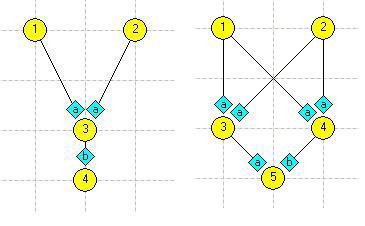
\includegraphics[width=0.85\textwidth]{modelle}}
\caption{Die Abbildung zeigt links schematisch den Aufbau eines Barlow-Levick Modells und recht den eines Reichhardt-Hassenstein Modells. a steht dabei für erregende Synapsen und b für hemmende Synapsen. Hier wäre die Vorzugsrichtung von links nach rechts. Die gelben Kreise repräsentieren Neurone.}
\label{modelle}
\end{figure}



\section{Material und Methoden}
\subsection{Material}
Für diesen Versuch benötigten wir lediglich einen Computer mit der Software Neurosim. 

\subsection{Versuchsaufbau}

\subsection{Versuchsdurchführung}

\section{Ergebnisse}
\subsection{Modul Goldmann}

\subsection{Modul Hodgkin - Huxley: Current Clamp}

\begin{table}[H]
\caption{Erhöhen des Stimulus bei 20 Grad C, ausgehend von $40.74\mu A$}
\centering
\begin{adjustbox}{width=1.3\textwidth, center=\textwidth}
\begin{tabular}{c|c|c}
Reizstrom in $\mu A$ & Zeit bis zur maximalen Spannung in ms & maximale Spannung in mV \\
\hline\hline
40.74 & 0.84 & 21.82\\
50.74 & 0.61 & 25.09\\
60.74 & 0.52 & 30.55\\
70.74 & 0.44 & 27.27\\
80.74 & 0.42 & 28.36\\
90.74 & 0.4 & 29.45\\
\end{tabular}
\end{adjustbox}
\end{table} 

\begin{figure}[H]
\makebox[\textwidth][c]{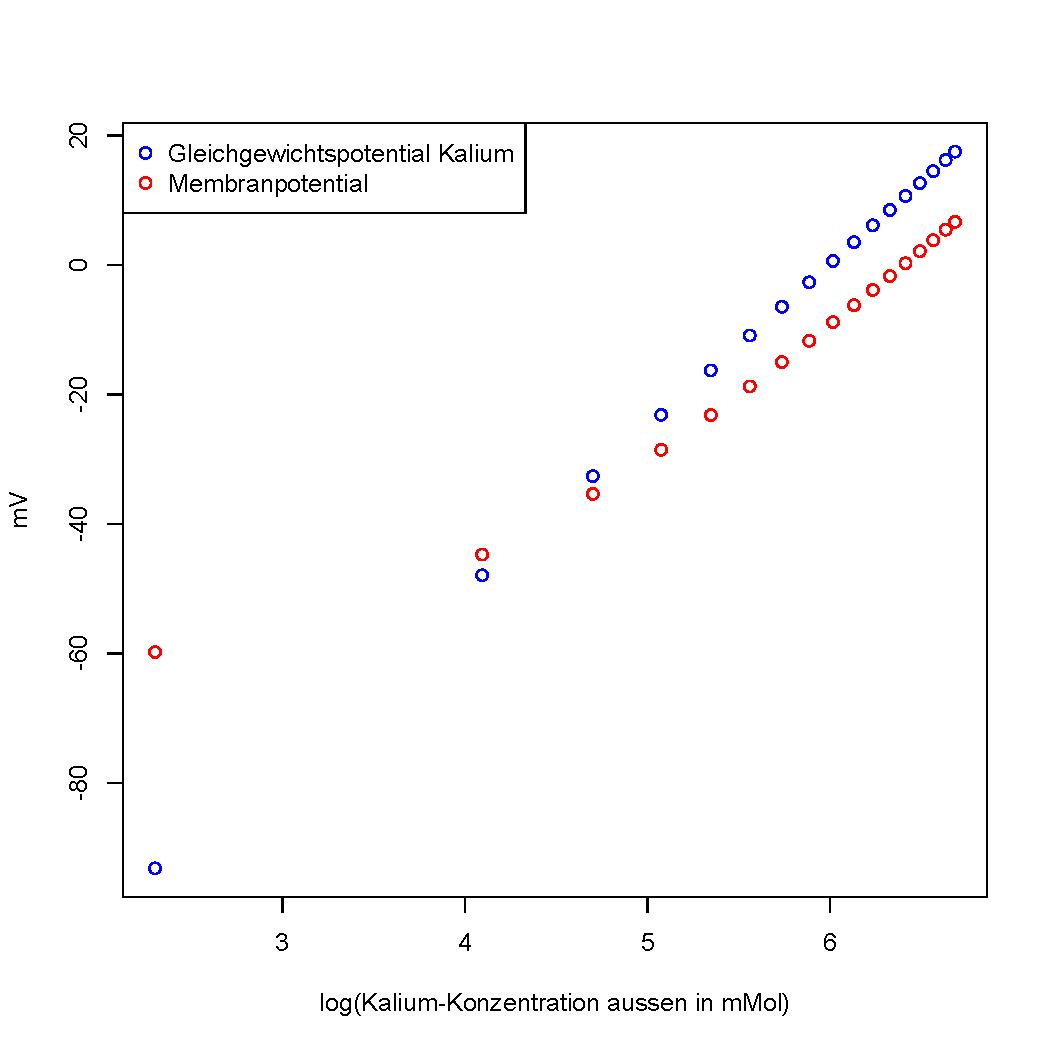
\includegraphics[width=\textwidth]{Aufgabe1/plot}}
\caption{Plot mit Graphen des Membranpotentials und des Gleichgewichtspotentials von Kalium in Abhängigkeit der Kalium-Konzentration außen (log-transformiert)}
\label{plot}
\end{figure}





\begin{table}[H]
\caption{Steigern des Reizstroms auf $130 \mu A$}
\begin{center}
\begin{tabular}{c|c|c}
Reizstrom in $\mu A$ & AP pro 100ms & Entladungsfrequenz in Hz \\
\hline\hline
2	&	1	&	10	\\
2,02	&	2	&	20	\\
2,06	&	3	&	30	\\
2,08	&	4	&	40	\\
3	&	5	&	50	\\
5,4	&	6	&	60	\\
10	&	7	&	70	\\
16	&	8	&	80	\\
22	&	9	&	90	\\
30	&	9	&	90	\\
35	&	10	&	100	\\
40	&	10	&	100	\\
45	&	11	&	110	\\
55	&	12	&	120	\\
70	&	12	&	120	\\
75	&	13	&	130	\\
90	&	13	&	130	\\
95	&	14	&	140	\\
115	&	14	&	140	\\
120	&	1	&	10	\\
125	&	1	&	10	\\
130	&	1	&	10	
\end{tabular}
\end{center}
\label{werte}
\end{table}

\subsection{Modul Hodgkin - Huxley: Voltage Clamp}


\begin{table}[H]
\caption{Testen verschiedener Klemmspannungen bei $-100$ mV Haltespannung}
\centering
\begin{adjustbox}{width=1.3\textwidth, center=\textwidth}
\begin{tabular}{c|c|c}
Klemmspannung in $-100$ mV & maximaler Stromfluss K$^+$ & maximaler Stromfluss Na$^+$\\
\hline\hline
-50	&	94,41	&	-346,15	\\
-40	&	346,15	&	-1069,93	\\
-30	&	692,31	&	-1793,71	\\
-20	&	1132,87	&	-2230,77	\\
-10	&	1604,9	&	-2409,09	\\
0	&	2108,39	&	-2318,18	\\
10	&	2548,95	&	-2090,91	\\
20	&	2989,51	&	-1608,39	\\
30	&	3398,6	&	-1013,99	\\
40	&	3870,63	&	-363,64	\\
50	&	4248,25	&	342,66	
\end{tabular}
\end{adjustbox}
\label{werte}
\end{table}


\subsection{Bewegungswahrnehmung}

\end{document}
